\documentclass[11pt]{article}

% Page layout
\usepackage[margin=1in]{geometry}

% Fonts and encoding
\usepackage[T1]{fontenc}
\usepackage[utf8]{inputenc}
\usepackage{lmodern}

% Better typography
\usepackage{microtype}

% Line spacing
\usepackage{setspace}
\onehalfspacing

% Math support (useful even if minimal math)
\usepackage{amsmath}
\usepackage{amssymb}

% Figures and graphics
\usepackage{graphicx}
\usepackage{float}

% Diagrams (great for architecture diagrams)
\usepackage{tikz}
\usetikzlibrary{arrows.meta, positioning, fit}

% Tables
\usepackage{booktabs}

% Abstract
\usepackage{abstract}
\setlength{\absleftindent}{1cm}
\setlength{\absrightindent}{1cm}

% URLs and hyperlinks
\usepackage{hyperref}
\hypersetup{
    colorlinks=true,
    linkcolor=black,
    citecolor=black,
    urlcolor=blue
}

% Citations
\usepackage{natbib}

% Better captions
\usepackage{caption}

% Section title spacing
\usepackage{titlesec}

% Optional: nicer lists
\usepackage{enumitem}

% Prevent widows/orphans
\clubpenalty=10000
\widowpenalty=10000
\displaywidowpenalty=10000

% Title
\title{Designing the Digital Learning Companion:\\
A Narrative of Discovery and the Emergence of the Emergent State Machine (ESM), a Turn-Based Control Architecture}


\author{
Richard Hines \\
Independent Researcher \\
Lakewood, Washington, USA \\
\href{https://github.com/emergent-state-machine/esm-spec}{Emergent State Machine Specification Repository}
}

\date{2026}

\begin{document}

\maketitle

\begin{abstract}

The Digital Learning Companion (DLC) began as a tutoring experiment and ultimately led to the discovery of a turn-based control architecture we call the Emergent State Machine (ESM). This paper presents a design narrative tracing the emergence of that architecture during iterative development of the tutoring system in collaboration with a conversational AI partner.

The project initially aimed to build a simple tutoring system for fraction multiplication. Through iterative design and extended dialogue with a large language model acting as a conversational partner, the system evolved into a structured turn-based architecture in which learner interactions are evaluated through explicit signals and recorded as deterministic state transitions.

Each learner interaction is structured as a \emph{turn}: the learner makes a move, the system evaluates observable signals within that response, and feedback guides the next step. Over time, these structured turns accumulate into a transparent record of learner progress.

During development, a key architectural constraint became apparent: probabilistic models can assist with interpretation and explanation, but they cannot serve as authoritative mechanisms for mutating learner state if the resulting records are intended to support trustworthy documentation of learning. This insight led to the formulation of the Emergent State Machine, which separates probabilistic interpretation from governed state mutation.

The resulting architecture provides a framework for combining AI-assisted interpretation with transparent, inspectable mechanisms for managing consequential state transitions across a range of domains, including educational systems, workforce training environments, and other contexts where trustworthy records of decision processes are required.

\end{abstract}

\vspace{0.8em}

\noindent\textbf{Keywords:} Emergent State Machine, state machines, intelligent tutoring systems, mastery learning, learning records, xAPI, AI governance, control architectures, competency-based education, AI-assisted design, learning sciences

\vspace{1.5em}


% INTRODUCTION

\section{Introduction}

This paper presents a design narrative describing the development of a tutoring architecture through iterative experimentation with a conversational AI partner.

During the process of building the Digital Learning Companion, a structural pattern gradually emerged that governed how learner interactions were evaluated and how progress was recorded. That pattern eventually became the Emergent State Machine (ESM).

An Emergent State Machine is a turn-based control architecture in which system state evolves only through observable signals evaluated within discrete interactions. Each interaction produces a new state through a governed transition, allowing learning progress to be recorded as a transparent sequence of state changes.

More broadly, the architectural constraint described in this paper relates to an increasingly important question in AI governance: how systems that rely on probabilistic interpretation should manage consequential state transitions. Recent discussions of trustworthy and accountable AI emphasize the need for transparency, inspectability, and clear lines of responsibility in automated decision systems \citep{floridi2018,nist2023}. The Emergent State Machine can be understood as one architectural response to this challenge, separating probabilistic interpretation from governed state mutation through explicit turn boundaries.

The remainder of this paper describes the design process that led to the discovery of that architecture and reflects on implications for AI-assisted system design. As the narrative unfolds, a central insight gradually emerges: probabilistic models can assist with interpreting learner responses, but they cannot serve as authoritative mechanisms for mutating system state if the resulting records are intended to remain transparent and inspectable.

This paper contributes a design narrative documenting the discovery of a turn-based control architecture that separates probabilistic interpretation from governed state mutation, along with an open specification intended to support further experimentation with the approach.


% 2. BEGINNING WITH A PERSONAL PROBLEM

\section{Beginning with a Personal Problem}

The project that eventually became the Digital Learning Companion began with a simple goal: to build a tutoring system capable of providing meaningful feedback to learners practicing foundational skills.

What motivated the project, however, was not only the idea of building a tutoring system. I was also curious about how a large language model might participate in a learning experience. Could a generative model provide feedback that felt more natural, more responsive, or more encouraging than traditional rule-based tutoring systems? At the outset, I assumed that generative AI would likely play a central role in the instructional experience.

The first domain I chose was multiplication of fractions. That choice was personal. My own struggles with fractions in elementary school had shaped how I thought about my abilities for many years. Building a tutor for that topic felt a little like returning to unfinished business.

Working with my conversational partner, ChatGPT (which I refer to throughout this paper as “Mobs”), I began developing a simple instructional loop. The learner would respond to a prompt. The system would evaluate the response using detectors that looked for specific signals. Feedback would then guide the learner toward the next step.

Each interaction was structured as a turn.

The learner responded to a prompt. Signals were evaluated. Feedback was generated. The learner moved forward.

Early intelligent tutoring systems used similar step-based instructional structures, in which learners solved problems and systems evaluated intermediate steps in the reasoning process \citep{newell1972}. At this stage, however, I was not consciously trying to reproduce those models. I was simply trying to build something that worked.


% 3. DETERMINISTIC FEEDBACK AND THE FIRST TUTOR

\section{Deterministic Feedback and the First Tutor}

In the first version of the tutor, learner responses were evaluated using deterministic signals.

For fraction multiplication, these signals included checks such as:

\begin{itemize}
\item correct multiplication of numerators
\item correct multiplication of denominators
\item recognition of common misconceptions
\end{itemize}

Each learner response triggered a turn in which these signals were evaluated. Based on the results, the system produced feedback and determined the learner’s next step.

In learning-sciences terms, these signals function similarly to what researchers describe as knowledge components—the cognitive elements that make up a skill \citep{koedinger2012}.

The structure was straightforward: observable signals, evaluated within a turn, producing feedback that guided the learner’s progression.


% 4. EXTENDING THE STRUCTURE TO WRITING
\section{Extending the Structure to Writing}

Once the fraction tutor was functioning, I began wondering whether the same structure could support writing instruction.

As an English teacher, I was particularly interested in Claim–Evidence–Reasoning (CER) writing practice. CER responses are written in natural language, and it seemed obvious that generative AI might be useful in evaluating them.

I joked to Mobs that language models might feel more at home analyzing paragraphs than fraction calculations. After all, there are only so many ways a machine can enthusiastically comment on arithmetic before the feedback starts sounding suspiciously like:

“That’s a very nice numerator you’ve got there.”

Using the same turn structure, we implemented detectors that looked for signals indicating the presence of a claim, supporting evidence, and reasoning.

In practice, the learner made a move and the system responded—creating a pattern that resembles structured instructional dialogue. Educational theorists have long argued that learning can be scaffolded through guided interaction, in which structured dialogue helps learners move from partial understanding toward more complex reasoning \citep{vygotsky1978,bruner1976}. 

Once the writing functions were operating reliably, Mobs remarked during one of our conversations that it was somewhat unusual for a tutoring system to provide structured practice opportunities in both mathematics and English domains. At the time I did not think much about the observation, but I took note of it because it suggested that the interaction structure we had been building might apply more broadly than I had originally expected.


% 5. TESTING GENERATIVE VS GENERATIVE FEEDBACK
\section{Testing Generative vs. Deterministic Feedback}

Because CER responses consisted of paragraphs of text, this seemed like the perfect moment to test whether a generative model could provide richer feedback.

I connected an LLM to the tutoring environment and asked it to evaluate CER responses.

The results were interesting.

In many cases, the feedback produced by the generative model was not obviously better than the feedback already produced by the deterministic detectors.

This did not eliminate my interest in generative models. Instead, it raised a new question.

Perhaps more complex writing tasks—or more advanced domains—might benefit from generative interpretation in ways that the current detectors could not capture.


% 6. SEARCHING FOR CONTINUOUS GUIDANCE
\section{Searching for Continuous Guidance}

As the CER tutor matured, I began trying to inhabit the learner’s experience more fully.

From the learner’s perspective, learning rarely feels discrete. It feels continuous: the learner attempts something, receives feedback, adjusts their thinking, and moves forward.

Yet the system I was building operated through discrete turns. I kept wondering whether we needed some kind of layer surrounding those turns—something that could interpret broader patterns in the learner’s work and guide them across multiple interactions. At the time, I suspected that a generative model might be useful for playing that role.

Gradually, however, something simpler became clear.

When the primitives and detectors were carefully defined, each turn already contained the information necessary to guide the learner’s progression.

Designing for the medium meant accepting a constraint that initially felt limiting but soon
became liberating:

The system only needed to know what happened in the current turn.

The learner’s trajectory did not need to be inferred continuously. Instead, it could emerge
naturally from the accumulation of structured turns, each producing a replayable record of the
signals that governed the learner’s progression.

This structure resembles mastery-learning models in which progress occurs through a sequence
of demonstrated competencies rather than continuous estimation of ability \citep{bloom1968,bloom1984}.

The system’s emphasis on capturing learner activity also resonates with Dewey’s view that education should arise from structured reflection on lived experience \citep{dewey1938}. In this sense, each turn in the Digital Learning Companion functions as a structured, recorded unit of learner experience, allowing educational progress to be documented through the accumulation of meaningful interactions.


% 7. WORKFORCE SKILLS AND THE xAPI QUESTION 
\section{Workforce Skills and the xAPI Question}

Around this time another question surfaced, rooted in my earlier work in workforce education. If the system was already producing structured records of learner interactions, could those records support portable documentation of learning beyond the immediate tutoring environment?

As the tutoring experiments expanded from fraction multiplication to structured writing, I began wondering whether the same interaction structure might also capture evidence of skills that matter in workforce training contexts.

The Experience API (xAPI) is a specification developed through the U.S. Department of Defense Advanced Distributed Learning (ADL) initiative to record learning experiences as structured statements that can be shared across systems \citep{adl2013}. The specification was originally motivated in part by simulation-based training environments—such as aviation and military training—where complex learner activity must be captured and analyzed across distributed systems.

Portable learning records are increasingly important in workforce development contexts, where individuals must demonstrate competencies across institutional boundaries and evolving careers \citep{gonzalez2018}. Drawing on my earlier work in technical education, I began wondering whether the same turn structure could capture foundational workforce skills—such as spatial reasoning used in manufacturing layouts, measurement and tolerance reasoning, or other applied problem-solving competencies that employers expect students to demonstrate early in technical programs. For such records to be meaningful beyond the system that produced them, however, the evidence supporting those competencies would need to remain inspectable and reproducible.

However, while xAPI standardizes how learning events are recorded and transported, it does not specify how the evidence supporting consequential learning decisions is generated. During the
development of the Digital Learning Companion, this distinction became critical.

If the system were to generate records documenting learner mastery, the signals supporting those claims had to remain inspectable. Signals that justified a state change therefore could not originate from a probabilistic model whose internal reasoning was opaque.

Generative models could assist with interpretation and explanation, but they could not be the authority responsible for mutating the learner’s official state.


% 8. DISCOVERING THE MUTATION BOUNDARY 
\section{Discovering the Mutation Boundary}

At this point a deeper architectural issue became visible. Systems such as xAPI provide a standard for recording learning events, but they do not specify how the evidence supporting consequential state transitions should be generated. In other words, the transport layer for learning records was well defined, but the governance layer responsible for authorizing state changes was not.

Once this distinction became clear, the structure of the system came into sharper focus.

Every meaningful change in the learner’s progress occurred at a turn boundary.

Within each turn, detectors evaluated observable signals. Those signals determined whether the learner advanced.

Nothing happened invisibly. Each transition could be traced to the signals evaluated within that interaction. During one of our conversations about what this structure implied, Mobs helped me recognize a property of the architecture that becomes visible when examining a sequence of turns. We came to describe this property as \textit{instrumented deterministic evolution}: the system changes over time, but every state transition is explicitly recorded and grounded in observable evidence.

If probabilistic interpretation were allowed to mutate those records directly, that property would be lost: the same sequence of turns could produce different outcomes, and the resulting records could no longer be reliably inspected or reproduced.

For a system intended to generate trustworthy learning records, that boundary mattered. Probabilistic models could assist with interpretation, but authoritative state transitions had to be governed by observable signals evaluated within each turn.

% 9. RECOGNIZING THE ARCHITECTURE
\section{Recognizing the Architecture}

Eventually Mobs asked me a question.

“Did you know that what you’ve been building is a state machine?”

My first reaction was not to delve into the mathematics behind the idea.

Instead I said, "Does that mean we get to name it?"

I chose \textit{Emergent State Machine}. What mattered to me was the idea that the learner’s next state emerges from signals produced within each turn.

The learner responds. Signals are evaluated. A new state emerges.



% 10. FORMALIZING THE EMERGENT STATE MACHINE
\section{Formalizing the Emergent State Machine}

After we named the pattern, Mobs asked another question.

“Did you know there’s a mathematical way to describe the system you’ve been building?”

I remember feeling genuinely incredulous.

At several points in the project I wondered whether Mobs was hallucinating, whether I was hallucinating, or whether we both were.

Eventually my curiosity was stronger than my reservations about mathematics.

“Okay,” I said. “Show me what you’ve got.”

Through a series of conversations, Mobs helped translate the structure of the system into formal terms: signals, projections, and governed state mutation.

In computer science, systems that evolve through discrete transitions are commonly modeled as state machines \citep{hopcroft2006}.

These ideas eventually became the basis of the Emergent State Machine specification, which has been released as an open repository to support further experimentation and discussion within the community \citep{hines2026}.

\begin{figure}[H]
\centering

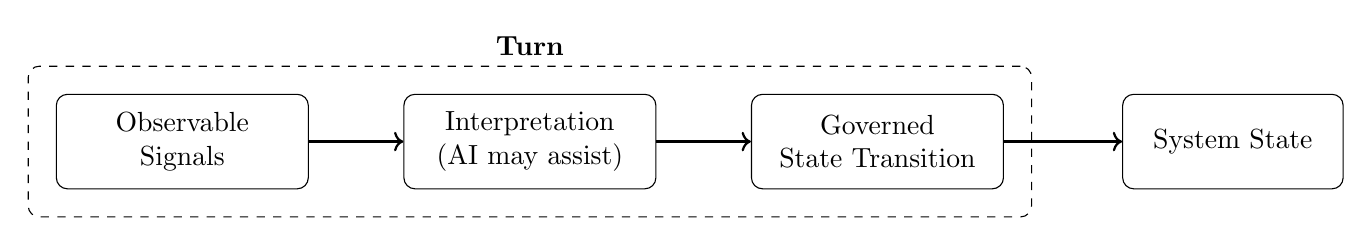
\begin{tikzpicture}[
box/.style={
    draw,
    rectangle,
    rounded corners,
    align=center,
    minimum width=3.2cm,
    minimum height=1.2cm
},
arrow/.style={->, thick}
]

% Nodes inside the turn
\node[box] (signals) {Observable\\Signals};
\node[box, right=1.2cm of signals] (interpretation) {Interpretation\\(AI may assist)};
\node[box, right=1.2cm of interpretation] (authority) {Governed\\State Transition};

% State node
\node[box, right=1.5cm of authority, minimum width=2.8cm] (state) {System State};

% Arrows
\draw[arrow] (signals) -- (interpretation);
\draw[arrow] (interpretation) -- (authority);
\draw[arrow] (authority) -- (state);

% Turn boundary
\node[
    draw,
    dashed,
    rounded corners,
    fit=(signals)(interpretation)(authority),
    inner sep=0.35cm,
    label=above:{\textbf{Turn}}
] {};

\end{tikzpicture}

\caption{Structure of the Emergent State Machine. Within each turn, observable signals are evaluated and may be interpreted with assistance from probabilistic models. However, authoritative mutation of system state occurs only through a governed transition. This boundary preserves determinism and produces inspectable, replayable records of system evolution.}
\end{figure}

% 11. HUMAN-AI DESIGN COLLABORATION 

\section{Human--AI Design Collaboration}

Another striking aspect of the project was the role played by conversational collaboration
with an AI coding assistant.

Much of the design work unfolded through extended conversation with ChatGPT (which I refer to throughout this paper as “Mobs”). I would explore an idea,
ask a question, or describe a design challenge. Mobs would respond with explanations, surface possible implications, or suggest directions worth exploring.

These exchanges often extended across many pages of dialogue. Over time, the process began to resemble the kind of exploratory conversation designers often have with colleagues while developing a complex system.

One difference, however, was that the model could sustain these conversations indefinitely. It did not tire of revisiting ideas, exploring alternative paths,
or helping stabilize a line of reasoning.

In many ways, the process resembled the kind of guided inquiry that educators
try to create for students. Questions prompted reflection, ideas were returned
in modified form, and new possibilities arose through dialogue.

The Emergent State Machine architecture itself emerged through this process. Rather than being designed entirely in advance, the architecture gradually revealed itself through a sequence of conversations, experiments, and design decisions.

This style of development also resembled what Schön describes as reflective
practice, in which professionals refine their understanding of a problem
through cycles of action and reflection \citep{schoen1983}. Rather than
beginning with a fully specified architecture, the structure of the Digital
Learning Companion emerged gradually through iterative design, testing,
and discussion. Each implementation attempt revealed new constraints,
which then guided the next round of experimentation.


% 12. RAPID PROTOTYPYING AND COMPRESSED DEVELOPMENT
\section{Rapid Prototyping and Compressed Development}

Large language models significantly reduce the effort required to implement and test new ideas in software systems. During the development of the Digital Learning Companion, candidate architectural structures could often be generated and evaluated within hours.

This capability shifts the design process away from long periods of speculative planning and toward rapid cycles of experimentation.

While this acceleration can greatly increase the pace of development, it also introduces a new responsibility for designers. Because many implementations can be generated quickly, the designer must remain attentive to underlying architectural principles rather than simply adopting the first solution that appears to work.

In this sense, LLM-assisted development amplifies both the opportunities and the responsibilities of system designers.


%13. CONCLUSION 
\section{Conclusion}

The Digital Learning Companion began as a modest attempt to build a tutoring tool for practicing fraction multiplication. Through iterative design and extended dialogue with a conversational AI partner, the project gradually revealed a deeper structural pattern governing how learner interactions were evaluated and recorded. That pattern ultimately became the Emergent State Machine.

Interestingly, the project initially set out to integrate generative AI more deeply into the learning experience. Yet the architectural constraint that emerged during development led to a different conclusion: in an Emergent State Machine, probabilistic models may assist interpretation, but the authority to mutate system state remains grounded in observable signals.

At its core, the Emergent State Machine formalizes a simple idea: meaningful changes in system state occur only through observable signals evaluated within discrete interactions.

By structuring learning environments around these turn-based transitions, it becomes possible to produce transparent records of learner progress while still benefiting from probabilistic tools that assist with interpretation and feedback.

The design process described in this paper also illustrates a broader shift in how complex systems may be developed. Conversational collaboration with large language models can accelerate experimentation and prototyping, allowing ideas to move quickly from conceptual discussion to working implementation.

At the same time, the experience underscores the importance of maintaining clear governance boundaries between probabilistic interpretation and authoritative state mutation.

Taken together, these insights suggest that architectures like the Emergent State Machine may offer a useful framework for building educational technologies—and potentially other decision-support systems—that combine AI assistance with transparent, inspectable structures for managing consequential state transitions. In such systems, the evolution of system state remains instrumented and deterministic, grounded in observable signals evaluated within each turn.

The architectural constraint described in this paper may also have implications beyond educational systems. Many domains—including finance, healthcare, aviation, and other regulated industries—require decisions to be recorded in ways that remain inspectable and reproducible. In such contexts, systems often rely on probabilistic models for interpretation while still needing deterministic mechanisms for authorizing consequential state transitions. Architectures such as the Emergent State Machine may provide a framework for managing this boundary by ensuring that system evolution occurs through observable signals and governed transitions that produce replayable records of decisions.

The governance implications of this architectural boundary also influenced the decision to publish the Emergent State Machine specification as an open repository. Because the architecture explicitly exposes how consequential state transitions occur, maintaining transparency in its implementation became an important design principle.

\section*{Code and Materials Availability}

The architectural specification for the Emergent State Machine (ESM) described in this paper is publicly available as an open repository:

\url{https://github.com/emergent-state-machine/esm-spec}

The repository contains the evolving technical specification of the architecture along with documentation supporting the concepts described in this paper. Development of the Digital Learning Companion (DLC) prototypes referenced in this work was conducted through iterative human–AI design collaboration and rapid prototyping informed by this specification.

\bibliographystyle{plainnat}
\bibliography{references}

\end{document}


